In this section, we present a theoretical performance prediction model
for \mad that estimates the total execution time of the
commissionning of a given assembly, according to the execution time of
each transition. Three goals are pursued with such a tool. First, the
theoretical execution time offers a way to evaluate the quality of the
prototype of \mad. Second, for a system administrator or a developer,
knowing the theoretical execution time of the commissioning procedure
is useful. Third, in the case of a fully autonomic commissioning and
reconfiguration process, which is left to future work, theoretical
information on the execution time is needed to take adequate
decisions, in particular for critical systems and services.

To build this performance prediction model, we need an estimation of
the execution time of all the actions in the assembly, given as a
function $time\,:\,\actions\rightarrow\mathbb{R}^+$.  Computing
precise execution times for the kind of actions used in a deployment
can be difficult and is itself the subject of many studies, \eg using
an analytical model or a statistical approach. However, for our
application, we find that estimates are sufficient as long as they preserve
the relative difference between different transitions.
%
Intuitively, we automatically deduce the execution flow of a \mad
assembly based on \mad' formal semantics. This is done by generating a
dependency graph representing the execution flow of each \mad
component in the assembly and connecting them together according to their
dependencies (the connections between their ports). Then, a
\emph{source} vertex is connected to the vertices representing the beginning of
the execution of each component, and a \emph{sink} vertex is connected to
the vertices representing the end of the execution of each component.
%
Thus, a dependency graph representing the execution of the whole
assembly is obtained. By weighting the arcs corresponding to the transitions with
the individual execution times of their actions (and the other ones with 0),
we can compute the expected total execution time of the assembly as the
longest path from the \emph{source} vertex to the \emph{sink} vertex.

% By generating a graph modelling the execution flow of a \mad assembly,
% capturing both intra-component and inter-component dependencies, we
% reduce this problem to finding the longest path in a DAG.

\subsection{Assumptions}

The performance model given here is valid only for assemblies such
that any set of places bound to a provide port contains exactly one
place. If a provide port is bound to a set containing multiple
places, the requirement imposed by this binding is satisfied as soon
as one of the places is reached. The total time then depends on the
earliest time at which one of these places is reached, which cannot be
modeled as a longest path. In practice this is not a severe
restriction, as ports requirements very rarely include
disjunctions. Indeed, none of our use-cases relies on this
feature. However, we still consider the possibility of having multiple
sets (of one place) bound to a port. In this case, the port is enabled
when all the places are reached.

%% \MC{Préciser ici que dans la pratique ce n'est pas un problème ?}
%% \HC[Maverick et Simon]{oui, j'ai commencé une phrase, il faut donner
%%   l'intuition du problème posé par la disjonction et aussi dire que
%%   dans la pratique sur des cas réels nous n'avons jamais eu besoin de
%%   disjonctions.}

The estimation provided by the model is a best case scenario: it
assumes that all actions are started as soon as possible, and that the
hardware has the capacity to run all possible parallel actions without
affecting their execution times.

%--------------------------------------
\subsection{Notations}
%--------------------------------------

%% Recall that given a component, we denote its set of places $\Pi$ and its
%% set of transitions $\Theta$. In the following, we consider that the
%% transitions go directly from a place to
%% another place instead of from an output dock to an input dock.
%% Hence, $\Theta$ is a multiset which elements are pairs of places.
%% \MC[Maverick,Simon]{Si on change les transitions pour qu'elles contiennent l'action,
%% plus besoin de parler de multiset je pense (+TODO ce ne sont plus des paires)}
%We
%can obtain the place corresponding to each dock by using the $place$
%function of the component.

%% We also consider the following two functions:
%% \begin{itemize}
%% \item the \emph{group entrance function} $g_{in}\,:\,G\rightarrow\mathcal{P}\left(\Pi\right)$ with\\
%% $g_{in}(g)=\left\{ \pi\,\mid\,\pi\in g\land\exists\pi_{b}\,:\,\left(\pi_{b}\not\in g\land\left(\pi_{b},\pi\right)\in\Theta\right)\right\} $
%% (the result of $g_{in}$ is called the set of \emph{entrance places}
%% of the group)
%% \item the \emph{group exit function} $g_{out}\,:\,G\rightarrow\mathcal{P}\left(\Pi\right)$ with\\
%% $g_{out}(g)=\left\{ \pi\,\mid\,\pi\in g\land\exists\pi_{a}\,:\,\left(\pi_{a}\not\in g\land\left(\pi,\pi_{a}\right)\in\Theta\right)\right\} $
%% (the result of $g_{out}$ is called the set of \emph{exit places}
%% of the group)
%% \end{itemize}

Recall that an assembly is a tuple $A = (C,L)$. In the following, for
any component $c_i \in C$, any of its associated set is denoted
$X_i$, \eg $\Pi_i$ for the set of places of the component $c_i$.  As
previously, for each set $X$ defining a component, we denote $X^*$ the
union (in the case of an assembly) or the extension (in the case of a
function) for all components. For instance
$\Pi^*=\bigcup_{i=1}^{n}\Pi_i$ denotes the set of all places in the
assembly.

The execution flow graph is an oriented weighted graph $\left(V,E\right)$
where $V$ is the set of vertices and $E$ is the set of weighted
arcs with elements in $V\times \mathbb{R}^{+} \times V$. We define
$V$ and $E$ in the following.

%--------------------------------------
\subsection{Vertices}
%--------------------------------------

For each place, we introduce two vertices: one representing the place
itself and one representing the event of a token leaving the place.
\[
V_{\Pi}=\bigcup_{\pi\in\Pi^*}\left\{ v_\pi^\text{place},v_\pi^\text{leav}\right\} 
\]
\MC[Maverick]{TODO : vérifier si on peut fusionner les deux sommets de
  place}
\HC[Maverick]{si c'est long a verifier, laisser comme ça, il faut
  qu'on soumette !}

For each transition, we introduce two vertices: one representing the
beginning of the transition and one representing its end.
\[
V_{\Theta}=\bigcup_{\theta\in\Theta^*}\left\{ v_\theta^\text{beg},v_\theta^\text{end}\right\} 
\]

\SR{On peut sans doute retirer les vertices representant les ports, et
  directement connecter $v^{place}_\pi$ à $v^{beg}_\theta$.}
\HC[Maverick et Simon]{oui je pense aussi, mais même remarque que au
  dessus, il faut qu'on soumette !}
For each provide port we introduce one vertex representing its enabling.
\[
V_{S_p}=\bigcup_{p\in S_p^*} \left\{ v_p^\text{start}\right\} 
\]


Finally, we define $V$ as the union of all these, plus one source
and one sink vertices. 
\[
V=V_{\Pi}\cup V_{\Theta} \cup V_{S_p} \cup \left\{ v^\text{source},v^\text{sink}\right\} 
\]

%--------------------------------------
\subsection{Arcs}
%--------------------------------------

In the dependency graph, arcs represent time constraints: the event represented
by the destination vertex must happen after the one represented by the source
vertex, at least $w$ seconds apart where $w$ is the weight of the arc. In
practice, arcs corresponding to actions are weighed with the corresponding
time, while other arcs have a weight 0 and merely represent a dependency.

For each place $\pi$ we introduce one arc from $v_\pi^\text{place}$ to
$v_\pi^\text{leav}$. This represents the fact that a token may leave $\pi$
only after it has entered it.
Figure~\ref{fig:place_graph} depicts the dependency graph corresponding to a place.
\[
E_{\Pi}=\bigcup_{\pi\in\Pi^*}\left\{ \left(v_\pi^\text{place},0,v_\pi^\text{leav}\right)\right\} 
\]

%%%%%%%%%%%%%%%
\begin{figure}[h]
  \subfloat[\mad place]{%
    \fcolorbox{black!20}{white}{
      \begin{minipage}[c][2.5cm][c]{0.43\linewidth}%
        \centering
        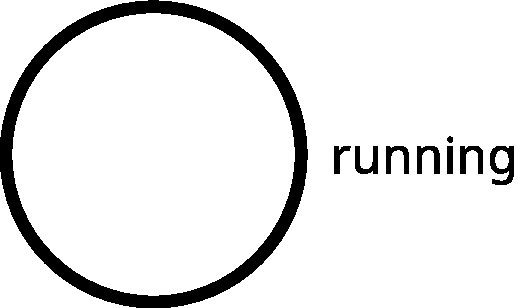
\includegraphics[scale=0.15]{images/perf_place.pdf}
      \end{minipage}
    }
  }
  \subfloat[Dependency graph]{%
    \fcolorbox{black!20}{white}{
      \begin{minipage}[c[c][2.5cm][c]{0.43\linewidth}%
        \centering
        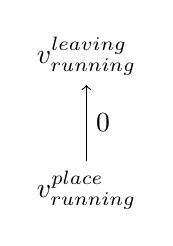
\begin{tikzpicture}[node distance=1.7cm]
          \node (leaving) [] {$v_\text{running}^\text{leaving}$};
          \node (place) [below of=leaving] {$v_\text{running}^\text{place}$};
          \draw [->] (place) -- (leaving) node[midway, right] {$0$};
        \end{tikzpicture}
      \end{minipage}
    }
  }
  \caption{A \mad place and its corresponding dependency graph}
  \label{fig:place_graph}
\end{figure}


For each transition $\theta = (s, \alpha, d)$, we introduce
three arcs. The first between $v_\theta^\text{beg}$ and $v_\theta^\text{end}$
represents the fact that the end of $\theta$ happens at the time of the
start of $\theta$ plus the time required for the action $\alpha$. The second between $v_{\pi(s)}^\text{leav}$
and $v_\theta^\text{beg}$ represents the fact that $\theta$ may only
happen after a token has left $\pi(s)$. The third one between $v_\theta^\text{end}$ and
$v_{\pi(d)}^\text{place}$ represents the fact that a token may enter $\pi(d)$ only
after $\theta$ has ended.
Figure~\ref{fig:transition_graph} depicts the dependency graph corresponding to three
transitions \emph{t1}, \emph{t2} and \emph{t3}.
\begin{align*}
E_{\Theta}=\bigcup_{\theta=(s,\alpha,d)\in\Theta^*} & \left\{ \left(v_\theta^\text{beg},time(\alpha),v_\theta^\text{end}\right),\right.\\
 & \left(v_{\pi(s)}^\text{leav},0,v_\theta^\text{beg}\right),\left. \left(v_\theta^\text{end},0,v_{\pi(d)}^\text{place}\right)\right\}
\end{align*}

%%%%%%%%%%%%%%%
\begin{figure}[h]
  \subfloat[\mad internal net example]{
    \fcolorbox{black!20}{white}{
      \begin{minipage}[c][7.5cm][c]{0.33\linewidth}%
        \centering
        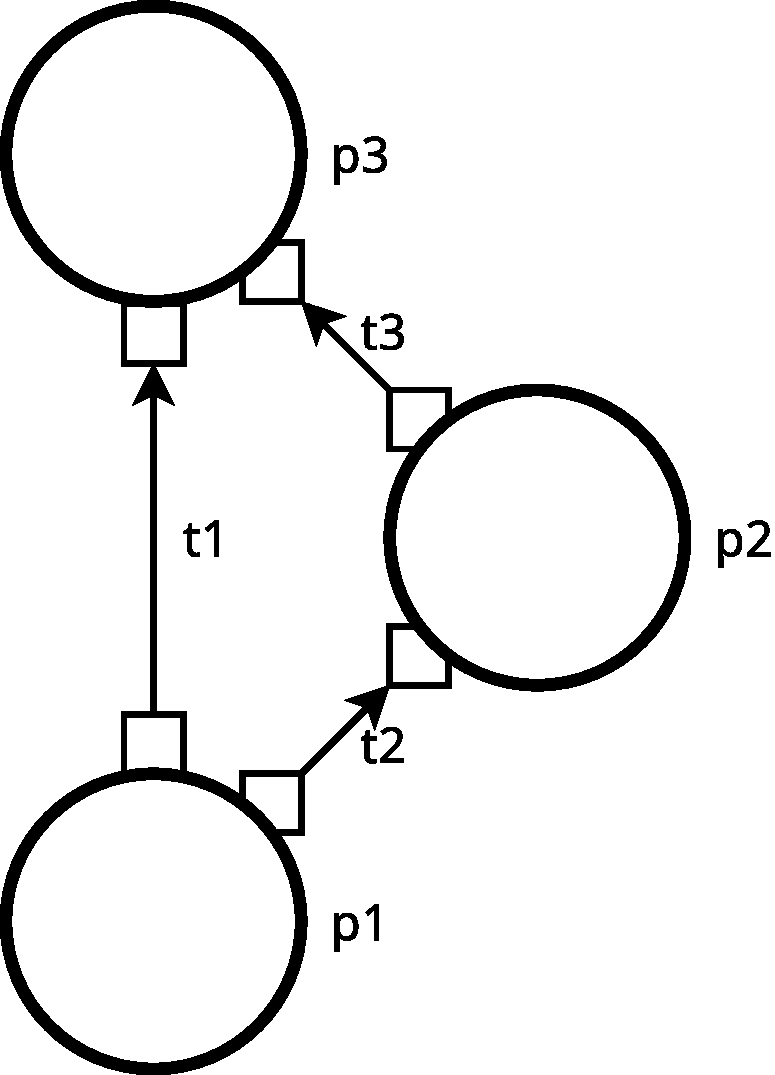
\includegraphics[width=0.8\columnwidth]{images/perf_transition.pdf} \label{fig:transmadeus}
      \end{minipage}
    }
  }
  \subfloat[Dependency graph]{
    \fcolorbox{black!20}{white}{
      \begin{minipage}[c][7.5cm][c]{0.53\linewidth}%
        \centering
        \begin{tikzpicture}[node distance=1.7cm]
          \node (p3l) [] {$v_\text{p3}^\text{leav}$};
          \node (p3) [below =15pt of p3l] {$v_\text{p3}^\text{place}$};
          \node (t1e) [below =15pt of p3] {$v_\text{t1}^\text{end}$};
          \node (t1) [below =15pt of t1e] {$v_\text{t1}^\text{beg}$};
          \node (p1l) [below =15pt of t1] {$v_\text{p1}^\text{leav}$};
          \node (p1) [below =15pt of p1l] {$v_\text{p1}^\text{place}$};
          \node (t2) [right =25pt of p1l] {$v_\text{t2}^\text{beg}$};
          \node (t2e) [right =25pt of t2] {$v_\text{t2}^\text{end}$};
          \node (p2) [above =15pt of t2e] {$v_\text{p2}^\text{place}$};
          \node (p2l) [above =15pt of p2] {$v_\text{p2}^\text{leav}$};
          \node (t3) [above =15pt of p2l] {$v_\text{t3}^\text{beg}$};
          \node (t3e) [right =15pt of p3] {$v_\text{t3}^\text{end}$};
          \draw [->] (p3) -- (p3l) node[midway, right, scale=0.7] {$0$};
          \draw [->] (p2) -- (p2l) node[midway, right, scale=0.7] {$0$};
          \draw [->] (p1) -- (p1l) node[midway, right, scale=0.7] {$0$};
          \draw [->] (t3) -- (t3e) node[midway, above, scale=0.7] {$time(\text{t3})$};
          \draw [->] (t2) -- (t2e) node[midway, below, scale=0.7] {$time(\text{t2})$};
          \draw [->] (t1) -- (t1e) node[midway, right, scale=0.7] {$time(\text{t1})$};
          \draw [->] (p1l) -- (t1) node[midway, right, scale=0.7] {$0$};
          \draw [->] (p1l) -- (t2) node[midway, below, scale=0.7] {$0$};
          \draw [->] (p2l) -- (t3) node[midway, right, scale=0.7] {$0$};
          \draw [->] (t1e) -- (p3) node[midway, right, scale=0.7] {$0$};
          \draw [->] (t2e) -- (p2) node[midway, right, scale=0.7] {$0$};
          \draw [->] (t3e) -- (p3) node[midway, above, scale=0.7] {$0$};
        \end{tikzpicture}
        \label{fig:transdag}
      \end{minipage}
    }
  }
  \caption{Example of a set of \mad transitions translated to its equivalent dependency graph}
  \label{fig:transition_graph}
\end{figure}


%% SR: text before modification
%% For each data-provide port $p$, we associate (a) for each binding between
%% $p$ and a place $\pi$ one arc from $v_\pi^\text{place}$ to
%% $v_p^\text{start}$, and (b) for each connection connecting $p$
%% to a data-use port $u$, for each binding between $u$ and a transition
%% $\theta$ one arc from $v_p^\text{start}$ to $v_\theta^\text{beg}$.

For each data-provide port $p$ and each place $\pi$ such that
$\{\pi\}$ is bound to $p$, we introduce one arc from
$v_\pi^\text{place}$ to $v_p^\text{start}$. This represents the
enabling of the port after all (set of) places bound to the port
have been reached.
\[
A_{S_p}= \bigcup_{(p,\{\pi\})\in B_{S_p}^*}\left\{ \left(v_\pi^\text{place},0,v_p^\text{start}\right)\right\}
\]

Additionally, for each provide port $p$ and each transition
$\theta$ such that $p$ is connected to a use port that is bound
to $\theta$, we introduce one arc from $v_p^\text{start}$ to
$v_\theta^\text{beg}$. This represents the activation of the transitions
bound to a use port, after the port is provided.
\[
E_{S_u} = \bigcup_{\substack{(u,p)\in L \\ (u,\theta)\in B_{S_u}^*}} \left\{ \left(v_p^\text{start},0,v_\theta^\text{beg}\right)\right\}
\]

Figure~\ref{fig:ports_graph} depicts the dependency graph corresponding to a
provide port \emph{p} bound to a place \emph{c1p} and connected to
a use port \emph{u} which is bound to a transition \emph{c2t}.
\SR[Maverick]{TODO: change figure (part a)}

%% SR: text before modification
%% Figure~\ref{fig:data_ports_graph} depicts the dependency graph corresponding to a
%% data-provide port \emph{dp} bound to a place \emph{c1p} and connected to
%% a data-use port \emph{du} which is bound to a transition \emph{c2t}.
%% \begin{align*}
%% A_{D}=\bigcup_{p\in D_p}
%% & \left(\bigcup_{\pi,\,\left(p,\pi\right)\in B_{D_{p}}^*}\left\{ \left(v_\pi^\text{place},v_p^\text{start},0\right)\right\}\right. \\
%% & \left.\cup\bigcup_{\substack{u,\,\left(u,p\right)\in L_D \\
%%   \theta,\,\left(u,\theta\right)\in B_{D_{u}}^*}}\left\{ \left(v_p^\text{start},v_\theta^\text{beg},0\right)\right\}\right)
%% \end{align*}

%%%%%%%%%%%%%%%
\begin{figure}[h]
  \subfloat[Madeus data connection]{%
    \fcolorbox{black!20}{white}{
      \begin{minipage}[c][5cm][c]{0.34\linewidth}%
        \centering
        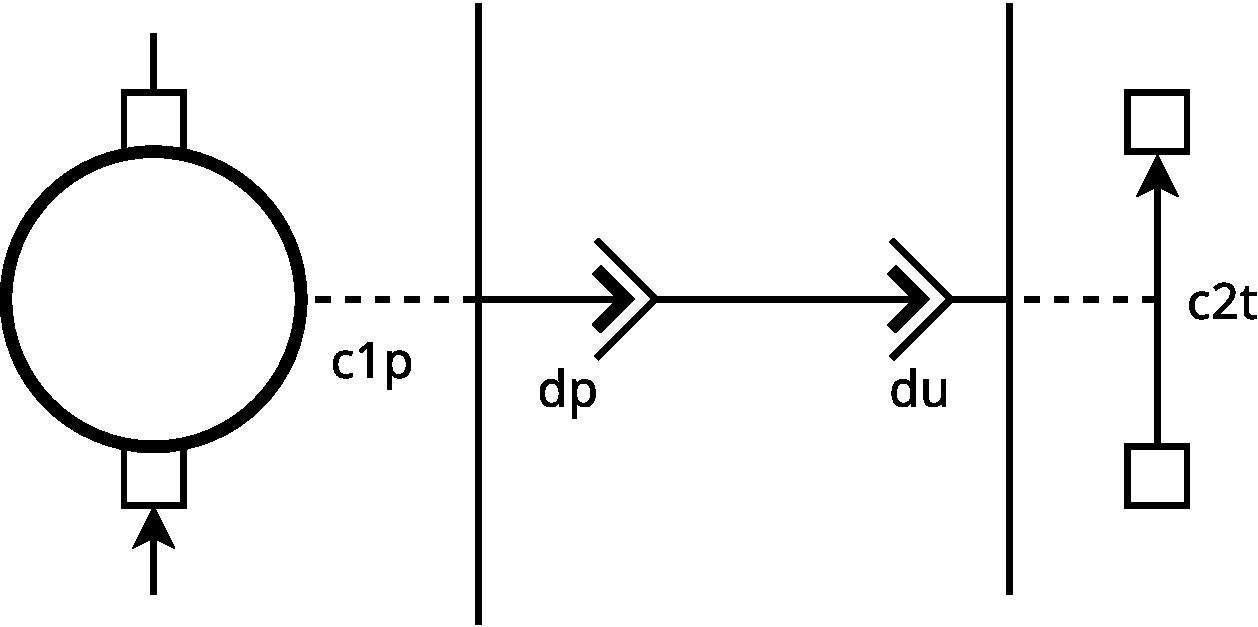
\includegraphics[scale=0.14]{images/perf_data_ports.pdf}
        \label{fig:port}
      \end{minipage}
    }
  }
  \subfloat[Dependency graph]{%
    \fcolorbox{black!20}{white}{
      \begin{minipage}[c][5cm][c]{0.52\linewidth}%
        \centering
        \begin{tikzpicture}[node distance=1.7cm]
          \node (c1t2) [] {$v_\text{c1t2}^\text{beg}$};
          \node (c1p1l) [below =15pt of c1t2] {$v_\text{c1p}^\text{leav}$};
          \node (c1p1) [below =15pt of c1p1l] {$v_\text{c1p}^\text{place}$};
          \node (c1t1_end) [below=15pt of c1p1] {$v_\text{c1t1}^\text{end}$};
          \draw [->] (c1t1_end) -- (c1p1) node[midway, right, scale=0.7] {$0$};
          \draw [->] (c1p1) -- (c1p1l) node[midway, right, scale=0.7] {$0$};
          \draw [->] (c1p1l) -- (c1t2) node[midway, right, scale=0.7] {$0$};
          \node (p) [right =15pt of c1p1] {$v_\text{p}^\text{start}$};
          \node (c2t) [right =15pt of p] {$v_\text{c2t}^\text{beg}$};
          \node (c2t_end) [above =15pt of c2t] {$v_\text{c2t}^\text{end}$};
          \draw [->] (c2t) -- (c2t_end) node[midway, right, scale=0.7] {$time(\text{c2t})$};
          \draw [->] (c1p1) -- (p) node[midway, below, scale=0.7] {$0$};
          \draw [->] (p) -- (c2t) node[midway, below, scale=0.7] {$0$};
        \end{tikzpicture}
        \label{fig:portdag}
      \end{minipage}
    }
  }
  \caption{A connection and its corresponding dependency graph}
  \label{fig:ports_graph}
\end{figure}


%% SR: text before modification (see below) 
%% For each service-provide port $p$, we associate (a) for each binding between
%% $p$ and a group $g$ one arc from $v_\pi^\text{place}$ to $v_p^\text{start}$
%% for each $\pi$ in $g_{in}(g)$ and one arc from $v_p^\text{stop}$ to
%% $v_\pi^\text{leav}$ for each place $\pi$ $g_{out}(g)$, and (b) for each
%% connection connecting $p$ to a service-use port $u$, for each binding between
%% $u$ and a transition $\theta$ one arc from $v_p^\text{start}$ to
%% $v_\theta^\text{beg}$ and one arc from $v_\theta^\text{end}$ to
%% $v_p^\text{stop}$.
%% The (a) arcs represent the fact that the service becomes available when all
%% groups bound to it have a token, and each of them can be deactivated only when
%% the provide port is not used anymore. The (b) arcs represent the
%% fact that the transitions bound to a service-use port may only execute once
%% the port is provided, and do not use the port anymore once they are over.

%% For each service-provide port $p$, each groupd $g$ bound to $p$ and
%% each place $\pi$ in $g_{in}(g)$, we introduce one arc from
%% $v_\pi^\text{place}$ to $v_p^\text{start}$, representing the
%% availability of the service once all groups bound to it hold a token.

%% Conversely, for each each service-provide port $p$, each group $g$
%% bound to $p$ and each place $\pi$ in $g_{out}(g)$, we introduce one
%% arc from $v_p^\text{stop}$ to $v_\pi^\text{leav}$, in order to
%% represent the fact that the group $g$ may not be disabled while the
%% port is busy.

%% Lastly, for each service-provide port $p$ and each transition $\theta$
%% such that $p$ is connected to a service-use port bound to $\theta$, we
%% introduce one arc from $v_p^\text{start}$ to $v_\theta^\text{beg}$ and
%% one arc from $v_\theta^\text{end}$ to $v_p^\text{stop}$. They
%% represent the activation of the transitions bound to a service-use
%% port after it has been provided, and the release of the port after the
%% transition is over.

%% Figure~\ref{fig:service_ports_graph} depicts the dependency graph corresponding to a
%% service-provide port \emph{sp} bound to a group with \emph{c1p1} as entrance
%% place and \emph{c1p2} as exit place, and connected to service-use port
%% \emph{su} which is bound to transition \emph{c2t}.

%% \begin{alignat*}{3}
%% A_{S}=\bigcup_{p\in S_p}
%% & \left(\bigcup_{g,\,\left(p,g\right)\in B_{S_{p}}^*} \right. && \left. \left(\bigcup_{\pi\in g_{in}(g)} \left\{\left(v_\pi^\text{place},v_p^\text{start},0\right)\right\}\right.\right. \\
%% &&& \left. \cup\left.\bigcup_{\pi\in g_{out}(g)} \left\{\left(v_p^\text{stop},v_\pi^\text{leav},0\right)\right\}\right)\right. \\
%% & \left.\cup\bigcup_{\substack{u,\,\left(u,p\right)\in L_S \\
%%       \theta,\,\left(u,\theta\right)\in B_{S_{u}}^*}} \right. && \left. \left\{ \left(v_p^\text{start},v_\theta^\text{beg},0\right),\right.\right. \left.\left.\left(v_\theta^\text{end},v_p^\text{stop},0\right)\right.\Big\}\right.\Bigg)
%% \end{alignat*}

%%%%%%%%%%%%%%%
%%\begin{figure}[t]
  \subfloat[\mad use-provide connection]{%
    \fcolorbox{black!20}{white}{
      \begin{minipage}[c]{0.95\columnwidth}%
        \centering
        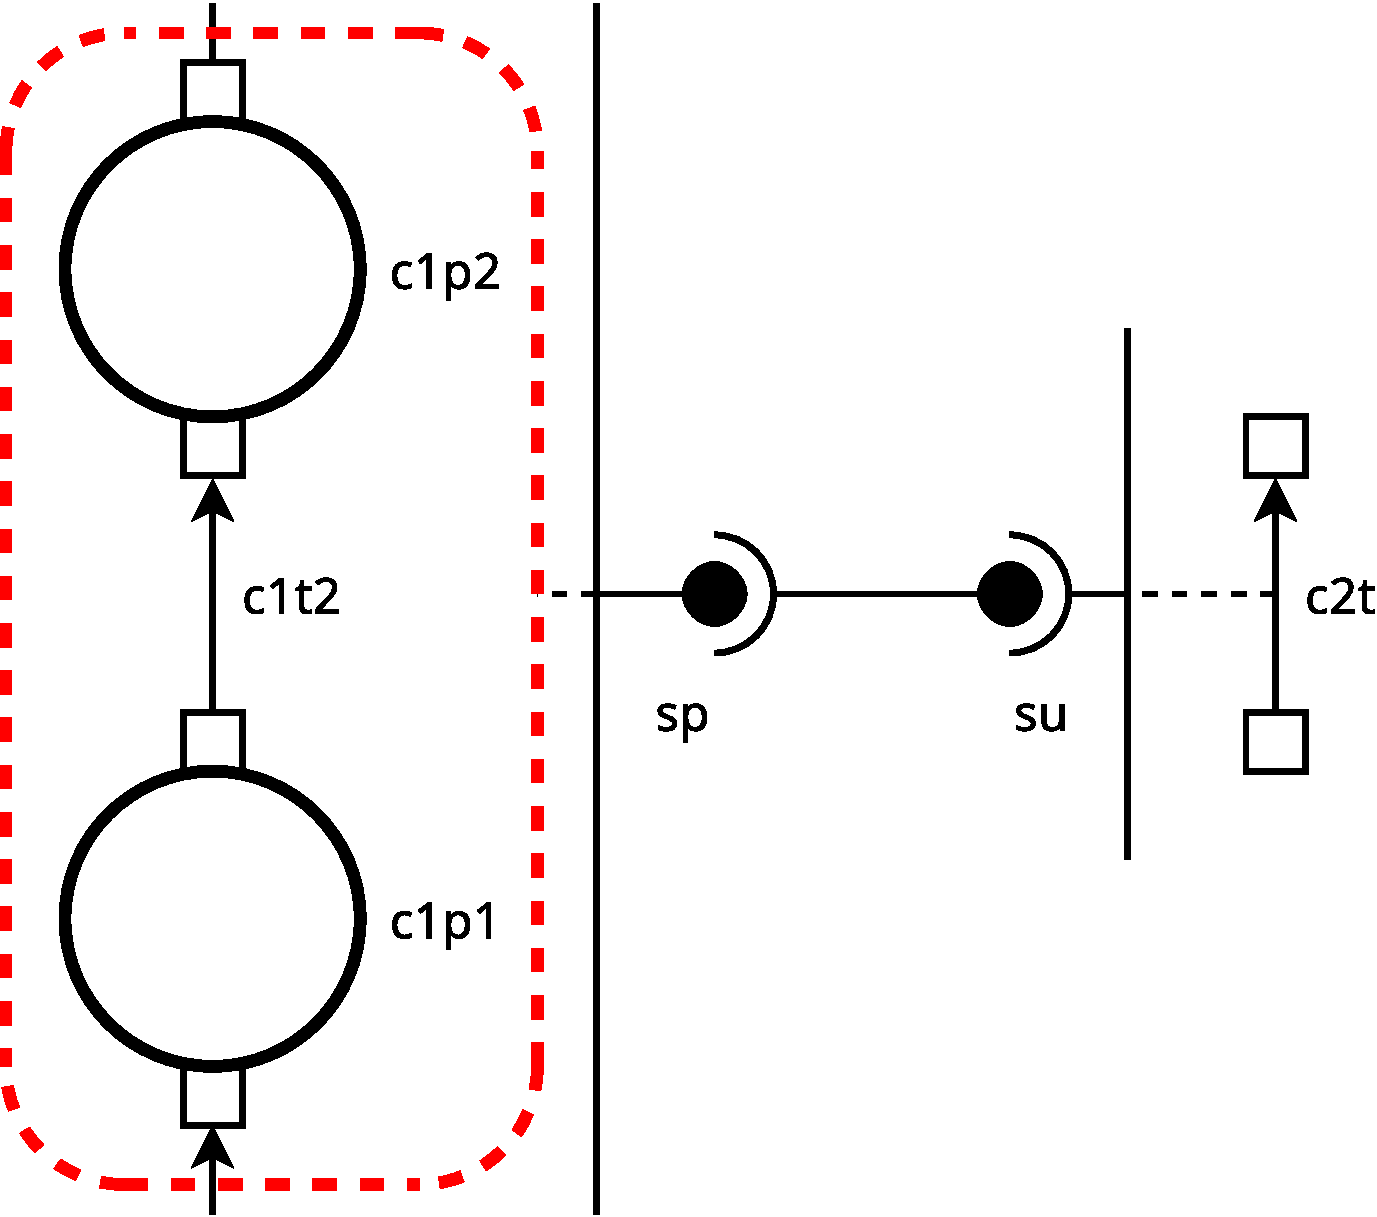
\includegraphics[scale=0.15]{images/perf_service_ports.pdf}
      \end{minipage}
    }
  }
  \\

  \subfloat[Dependency graph]{%
    \fcolorbox{black!20}{white}{
      \begin{minipage}[c]{0.95\columnwidth}%
        \centering
        \begin{tikzpicture}[node distance=1.7cm]
          \node (c1t3) [] {$v_\text{c1t3}^\text{beg}$};
          \node (c1p2l) [below =15pt of c1t3] {$v_\text{c1p2}^\text{leav}$};
          \node (c1p2) [below =15pt of c1p2l] {$v_\text{c1p2}^\text{place}$};
          \node (c1t2_end) [below =15pt of c1p2] {$v_\text{c1t2}^\text{end}$};
          \node (c1t2) [below =15pt of c1t2_end] {$v_\text{c1t2}^\text{beg}$};
          \node (c1p1l) [below =15pt of c1t2] {$v_\text{c1p1}^\text{leav}$};
          \node (c1p1) [below =15pt of c1p1l] {$v_\text{c1p1}^\text{place}$};
          \node (c1t1_end) [below =15pt of c1p1] {$v_\text{c1t1}^\text{end}$};
          \draw [->] (c1t1_end) -- (c1p1) node[midway, right, scale=0.7] {$0$};
          \draw [->] (c1p1) -- (c1p1l) node[midway, right, scale=0.7] {$0$};
          \draw [->] (c1p1l) -- (c1t2) node[midway, right, scale=0.7] {$0$};
          \draw [->] (c1t2) -- (c1t2_end) node[midway, right, scale=0.7] {$time(\text{c1t2})$};
          \draw [->] (c1t2_end) -- (c1p2) node[midway, right, scale=0.7] {$0$};
          \draw [->] (c1p2) -- (c1p2l) node[midway, right, scale=0.7] {$0$};
          \draw [->] (c1p2l) -- (c1t3) node[midway, right, scale=0.7] {$0$};
          \node (sp) [right =20pt of c1p1] {$v_\text{sp}^\text{start}$};
          \node (c2t) [right =20pt of sp] {$v_\text{c2t}^\text{beginning}$};
          \node (c2t_end) [above =15pt of c2t] {$v_\text{c2t}^\text{end}$};
          \node (sps) [right =20pt of c1p2l] {$v_\text{sp}^\text{stop}$};
          \draw [->] (c2t) -- (c2t_end) node[midway, right, scale=0.7] {$time(\text{c2t})$};
          \draw [->] (c1p1) -- (sp) node[midway, below, scale=0.7] {$0$};
          \draw [->] (sp) -- (c2t) node[midway, below, scale=0.7] {$0$};
          \draw [->] (c2t_end) to[bend right] node[midway, right, scale=0.7] {$0$}(sps.east) ;
          \draw [->] (sps) -- (c1p2l) node[midway, above, scale=0.7] {$0$};
        \end{tikzpicture}
      \end{minipage}
    }
  }
  \caption{Vertices and arcs for service ports, bindings and connections}
  \label{fig:service_ports_graph}
\end{figure}

For each initial place $\pi$ we introduce one arc from $v^\text{source}$
to $v_\pi^\text{place}$, representing the fact that a token is placed in each
initial place in the initial configuration.
Figure~\ref{fig:source_sink_graph} depicts the dependency graph corresponding to two initial
places \emph{c1p1} and \emph{c2p2}.
\[
E_I=\bigcup_{\pi, \Delta_i(\pi) = \emptyset}\left\{ \left(v^\text{source},0,v_\pi^\text{place}\right)\right\} 
\]

For each final place $\pi$ we introduce one arc from $v_\pi^\text{place}$
to $v^\text{sink}$. Intuitively, this represents the fact that the
commissionning is over only after all components have reached the
places without outgoing transitions.
Figure~\ref{fig:source_sink_graph} depicts the dependency graph
corresponding to three final places \emph{c1p2}, \emph{c2p2}
and \emph{c2p3}.
\[
E_F=\bigcup_{\pi, \Delta_o(\pi) = \emptyset}\left\{ \left(v_\pi^\text{place},0,v^\text{sink}\right)\right\} 
\]

%%%%%%%%%%%%%%%
\begin{figure}[t]
  \subfloat[\mad assembly]{%
    \begin{minipage}[c]{0.95\columnwidth}%
      \centering
      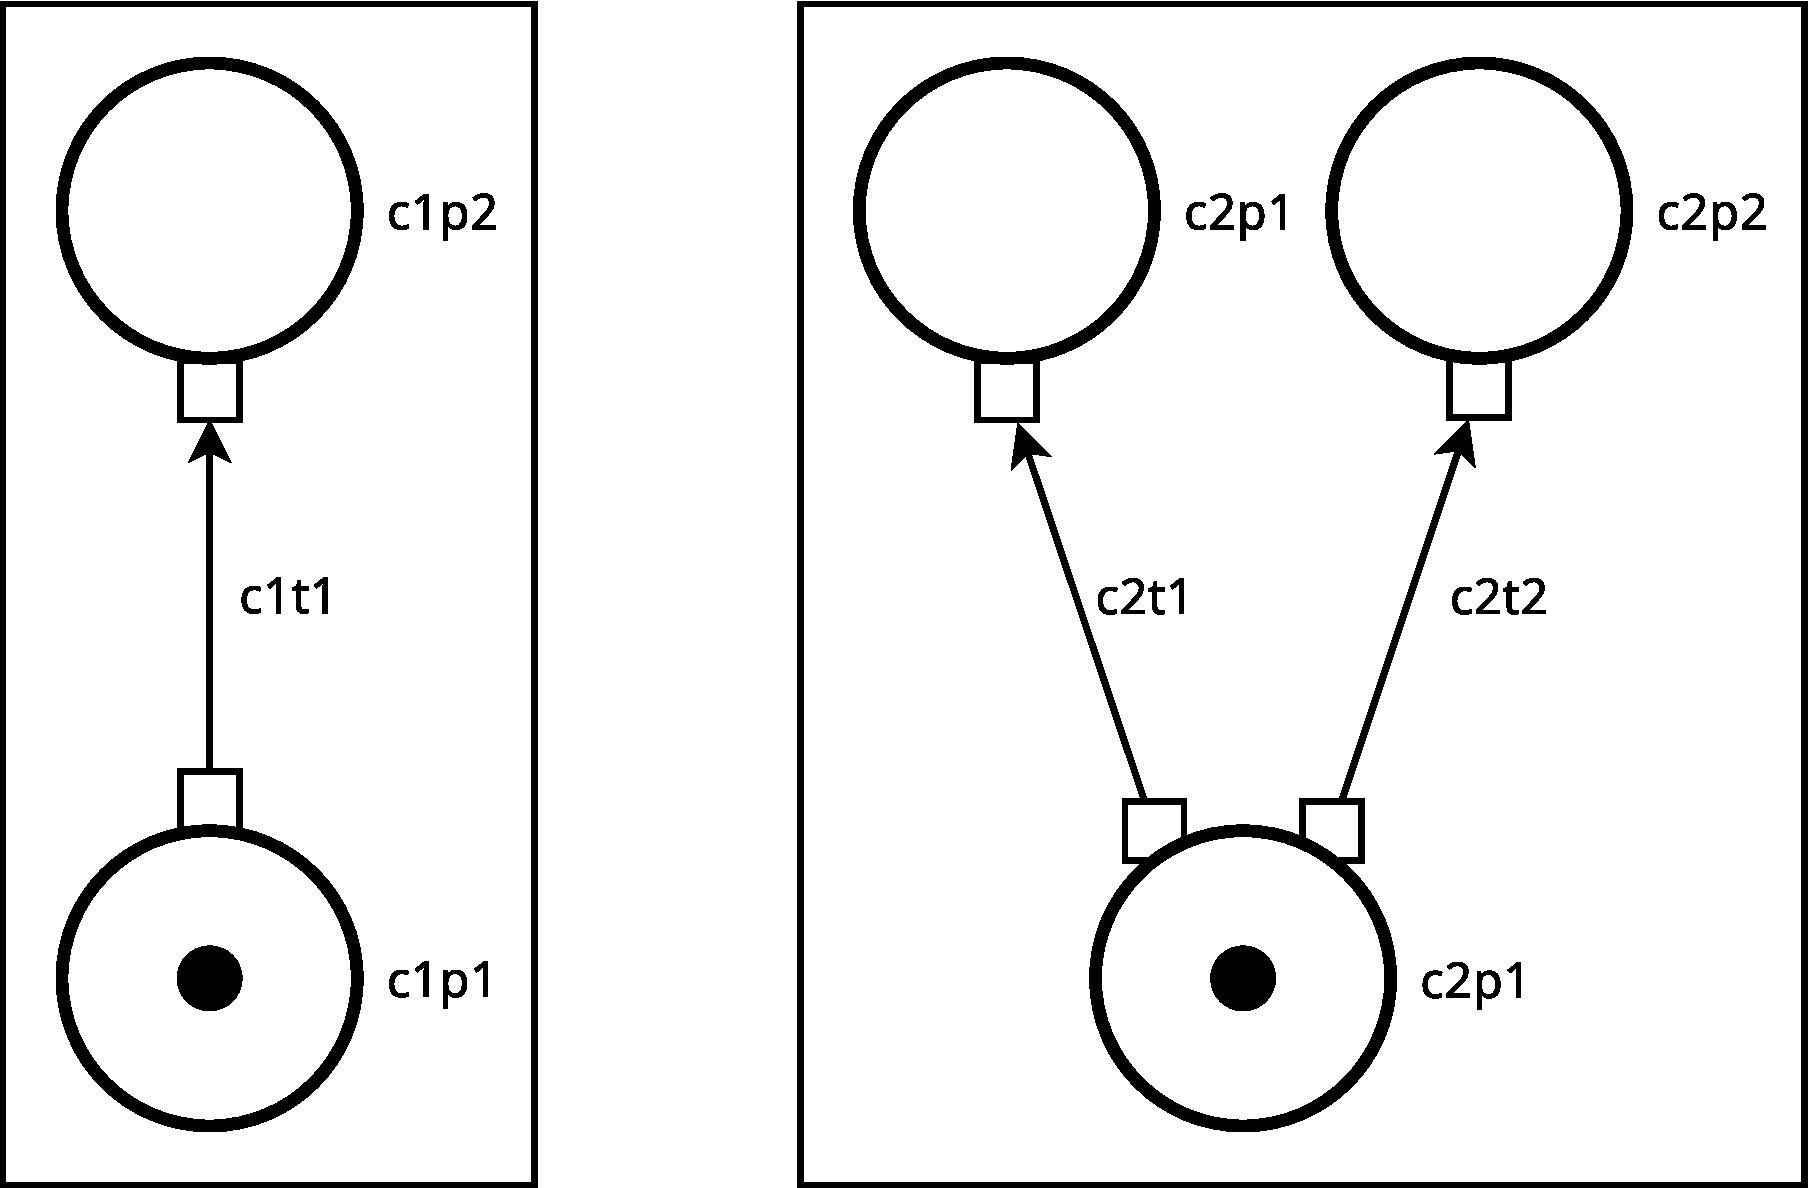
\includegraphics[scale=0.15]{images/perf_source_sink.pdf}
    \end{minipage}
  }
  \\
  
  \subfloat[Dependency graph]{%
    \fcolorbox{black!20}{white}{
      \begin{minipage}[c]{0.95\columnwidth}%
        \centering
        \begin{tikzpicture}[node distance=1.7cm]
          \node (c1p2l) [] {$v_\text{c1p2}^\text{leav}$};
          \node (c1p2) [below =15pt of c1p2l,yshift=-0.3cm] {$v_\text{p1p2}^\text{place}$};
          \node (c1t1e) [below =15pt of c1p2] {$v_\text{c1t1}^\text{end}$};
          \node (c1t1) [below =15pt of c1t1e] {$v_\text{c1t1}^\text{beg}$};
          \node (c1p1l) [below =15pt of c1t1] {$v_\text{c1p1}^\text{leav}$};
          \node (c1p1) [below =15pt of c1p1l] {$v_\text{c1p1}^\text{place}$};
          \node (c2p2) [right =35pt of c1p2] {$v_\text{c2p2}^\text{place}$};
          \node (c2p2l) [above =15pt of c2p2] {$v_\text{c2p2}^\text{leav}$};
          \node (c2t1e) [below =15pt of c2p2] {$v_\text{c2t1}^\text{end}$};
          \node (c2t1) [below =15pt of c2t1e] {$v_\text{c2t1}^\text{beg}$};
          \node (c2p1l) [below =15pt of c2t1, xshift=1.5cm] {$v_\text{c2p1}^\text{leav}$};
          \node (c2p1) [below =15pt of c2p1l] {$v_\text{c2p1}^\text{place}$};
          
          \node (c2p3) [right =35pt of c2p2] {$v_\text{c2p3}^\text{place}$};
          \node (c2p3l) [above =15pt of c2p3, yshift=0.3cm] {$v_\text{c2p3}^\text{leav}$};
          \node (c2t2e) [below =15pt of c2p3] {$v_\text{c2t2}^\text{end}$};
          \node (c2t2) [below =15pt of c2t2e] {$v_\text{c2t2}^\text{beg}$};
          
          \node (source) [below =15pt of c2p1, xshift=-1.8cm] {$v^\text{source}$};
          \node (sink) [above =20pt of c2p2l] {$v^\text{sink}$};
          
          \draw [->] (c1p1) -- (c1p1l) node[midway, right, scale=0.7] {$0$};
          \draw [->] (c1p2) -- (c1p2l) node[midway, right, scale=0.7] {$0$};
          \draw [->] (c2p1) -- (c2p1l) node[midway, right, scale=0.7] {$0$};
          \draw [->] (c2p2) -- (c2p2l) node[midway, right, scale=0.7] {$0$};
          \draw [->] (c2p3) -- (c2p3l) node[midway, right, scale=0.7] {$0$};
          \draw [->] (c1t1) -- (c1t1e) node[midway, right, scale=0.7] {$time(\text{c1t1})$};
          \draw [->] (c2t1) -- (c2t1e) node[midway, right, scale=0.7] {$time(\text{c2t1})$};
          \draw [->] (c2t2) -- (c2t2e) node[midway, right, scale=0.7] {$time(\text{c2t2})$};
          \draw [->] (c1p1l) -- (c1t1) node[midway, right, scale=0.7] {$0$};
          \draw [->] (c2p1l) -- (c2t1) node[midway, right, scale=0.7] {$0$};
          \draw [->] (c2p1l) -- (c2t2) node[midway, right, scale=0.7] {$0$};
          \draw [->] (c1t1e) -- (c1p2) node[midway, right, scale=0.7] {$0$};
          \draw [->] (c2t1e) -- (c2p2) node[midway, right, scale=0.7] {$0$};
          \draw [->] (c2t2e) -- (c2p3) node[midway, right, scale=0.7] {$0$};
          \draw [->] (source.west) to[bend left] node[midway, above, scale=0.7]{$0$} (c1p1.south);
          \draw [->] (source.east) to[bend right] node[midway, above, scale=0.7] {$0$}(c2p1.south);
          \draw [->] (c1p2) -- (sink) node[midway, right, scale=0.7] {$0$};
          \draw [->] (c2p2) to[bend right] node[midway, right, scale=0.7] {$0$}(sink);
          \draw [->] (c2p3) -- (sink) node[midway, right, scale=0.7] {$0$};
        \end{tikzpicture}
      \end{minipage}
    }
  }
  \caption{Transofrmation example fro mtwo components without ports to
    its equivalent execution flow graph}
  \label{fig:source_sink_graph}
\end{figure}

Finally, we define $E$ as 
\[
E=E_\Pi\cup E_{\Theta} \cup E_{S_p}\cup E_{S_u}\cup E_{I}\cup E_{F}
\]

%--------------------------------------
\subsection{Time estimation}
%--------------------------------------

In the following, we denote $DG_A=(V,E)$ the dependency graph corresponding
to assembly $A=(C,L)$, and $DG_c$ the part of a dependency graph
corresponding to component $c \in C$.

We define the time estimation of the execution of the \mad assembly $A$
to be the length of a longest path between $v^\text{source}$ and
$v^\text{sink}$ in $DG_A$.

\begin{lemma}
 In $DG_A$, if $v^\text{sink}$ is reachable from $v^\text{source}$ and there
 are no cycles, then the time estimation for $A$ is well-defined.
 \label{lemma:well_defined}
\end{lemma}

\begin{proof}
 If $v^\text{sink}$ is reachable from $v^\text{source}$, there exists at least
 one path from $v^\text{source}$ to  $v^\text{sink}$. Because there are no
 cycles, the number of paths between $v^\text{source}$ and $v^\text{sink}$ is
 finite. Because all the paths have a weight, the set of longest paths is
 well-defined (and not empty). Therefore the length of a longest path is
 well-defined.
\end{proof}

\begin{lemma}
 In a component $c \in C$, if place $\pi_t \in \Pi$ is reachable from place
 $\pi_s \in \Pi$ (distinct from $\pi_t$), then $v_{\pi_t}^{place}$
 is reachable from $v_{\pi_s}^{place}$ in a $DG_c$.
 \label{lemma:reachable}
\end{lemma}

\begin{proof}
 Consider a path $P$ in the \net of $c \in C$ from $\pi_s$ to
 $\pi_t$ (this path exists because $\pi_t$ is reachable from
 $\pi_s$). This path is made of a sequence of places connected by
 transitions: $P=(\pi_s,t1,p2,t2,\dots,t_n,\pi_t)$.\\
 By construction, there exists a path\\
 $(v_{\pi_s}^{place},v_{\pi_s}^{leav},v_{t1}^{beg},v_{t1}^{end},v_{p2}^{place},\dots,v_{\pi_t}^{place})
 \in DG_c$.
\end{proof}


\begin{lemma}
 If an assembly $A$ has one or more components then $v^\text{sink}$ is
 reachable from $v^\text{source}$ in $DG_A$.
 \label{lemma:source_sink}
\end{lemma}

\begin{proof}
 Let us consider one component $c \in C$, its initial place $\pi_i$ and one of
 its final places $\pi_f$. By construction, $v_{\pi_i}^\text{place}$ is
 reachable from $v^\text{source}$, and $v^\text{sink}$ is reachable from
 $v_{\pi_f}^\text{place}$ in the dependency graph of an assembly containing this
 component. The last thing to prove is that $v_{\pi_f}^\text{place}$ is reachable
 from $v_{\pi_i}^\text{place}$ in $DG_c$.
 The end of the execution of a \mad component is defined as
 when all its tokens are in final places, \ie when there are no more
 transitions to perform. Therefore, by definition $\pi_f$ is
 necessarily reachable from $\pi_i$ in the \net of $c \in C$.
 We conclude by applying Lemma~\ref{lemma:reachable}.
\end{proof}

\begin{lemma}
 If a component $c \in C$ is well-formed then $DG_c$ has no cycle.
 \label{lemma:no_cycles_component}
\end{lemma}

\begin{proof}
 By construction, in $DG_c$ the vertices and arcs corresponding to places do
 not form cycles and are disjoint, so they cannot produce a cycle by themselves.
 Likewise, the arcs corresponding to port bindings have either their source
 vertex or their destination vertex of degree 1, so they cannot produce a cycle.
 Only the arcs corresponding to transitions can produce cycles. Moreover, the
 arcs in $DG_c$ connect only the vertices corresponding to the places which
 are connected in the \net. This means that if there is a cycle in $DG_c$,
 there is a cycle in the \net. However, the \net of a well-formed \mad component
 has no cycle. Therefore there are no cycles in $DG_c$.
\end{proof}

\begin{lemma}
 In an assembly $A$ of well-formed components with no deadlocks, if each port
 is bound to at most one element (place, transition or group) and if
 $\left|g_{in}(g)\right|\leq 1$ and $\left|g_{out}(g)\right|\leq 1$ for each group
 $g$ in $A$ then the $DG_A$ has no cycles.
 \label{lemma:no_cycles_assembly}
\end{lemma}

\begin{proof}
 By Lemma~\ref{lemma:no_cycles_component}, we have that the dependency graph
 of all the components in $A$ have no cycles.
 Then, the only way a cycle may exist in $DG_A$ is if the vertices and arcs
 corresponding to connections cause a cycle to exist.
 This may be acheived in two ways: because of a single service port bound to
 group $g$ if $\left|g_{out}(g)\right|>0$ (which implies by hypothesis
 $\left|g_{out}(g)\right|=1$); or because of two or more use and provide ports.
 First, because $\left|g_{out}(g)\right|=1$ (we consider $\pi_{out}$ to be the only
 place in $g_{out}(g)$), and because by construction $v_{\pi_{out}}^{leav}$ is
 reachable from $v_{\pi_{in}}^{place}$ (where $\pi_{in}$ is the only place in $g_{in}(g)$,
 then $v_{\pi_{in}}^{place}$ is not reachable from $v_{\pi_{out}}^{leav}$ (otherwise
 there would be a cycle in the dependency graph of the component). Second, a
 cycle can be caused by multiple connections if there are \emph{crossing
 dependencies} (see Figure~\ref{fig:deadlock}). However, this would create a
 deadlock in the assembly, which is not possible by hypothesis.
\end{proof}

\begin{figure}[t]
  \begin{center}
    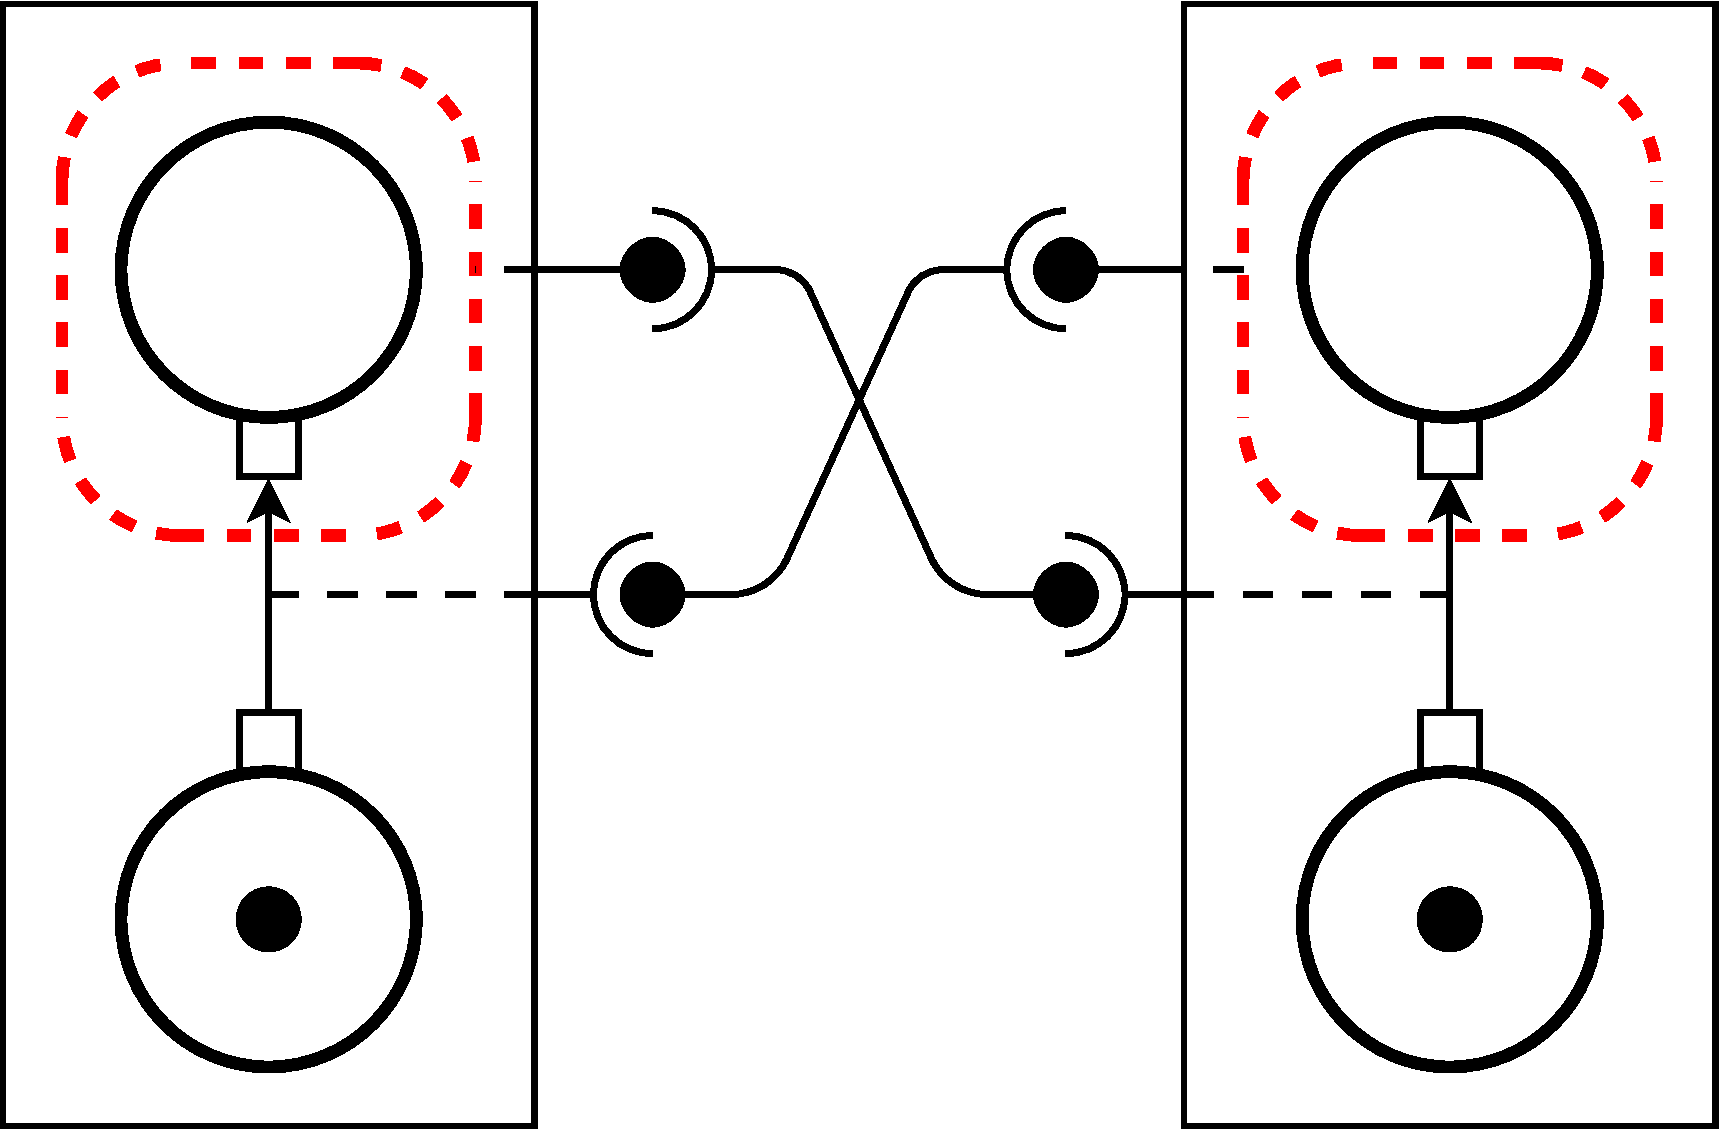
\includegraphics[width=0.5\linewidth]{./images/deadlock.pdf}
  \end{center}
  \caption{Example of an invalid assembly: crossing dependencies cause a deadlock.}
  \label{fig:deadlock}
\end{figure}

\begin{theorem}
 In an assembly $A$ of one or more well-formed components with no deadlocks,
 if each port is bound to at most one element (place, transition or group) and if
 $\left|g_{in}(g)\right|\leq 1$ and $\left|g_{out}(g)\right|\leq 1$ for each group
 $g$ in $A$, then the time estimation obtained using $DG_A$ is well-defined.
 \label{theorem:well_defined}
\end{theorem}

\begin{proof}
 By applying Lemma~\ref{lemma:source_sink}, we know that $v^\text{sink}$ is reachable
 from $v^\text{source}$. By applying Lemma~\ref{lemma:no_cycles_assembly}, we know
 that there are no cycles in $DG_A$. We conclude by applying
 Lemma~\ref{lemma:well_defined}.
\end{proof}

\paragraph{Remark}

The restrictions imposed in \ref{theorem:well_defined} are here to consider only
assemblies for which the structure of the dependency graph does not change
depending on the duration of the transitions. To handle arbitrary assemblies,
a more complex performance model is needed, which is left as future work. In
practice, we expect most real-life assemblies to fulfill these requirements.
In particular, all of the assemblies presented in this article do.


\subsection{Complexity}

We now determine the size complexity of $DG_A=(V,E)$ and the time
complexity of computing the time estimation.

First, we notice that
$|V| \in \mathcal{O}\left(\left|\pi^*\right|+\left|\theta^*\right|+\left|S_{p^*}\right|+\left|D_{p^*}\right|\right)$
and
$|E| \in \mathcal{O}\left(\left|\pi^*\right|+\left|\theta^*\right|+\left|B_{S_p}\right|+\left|B_{D_p}\right|+\left|B_{S_u}\right|\times\left|L_S\right|\right.$ \\
$\left.+\left|B_{D_u}\right|\times\left|L_D\right|\right)$
.

Because $DG_A$ is a a directed acyclic graph, finding the longest path
between $v^\text{source}$ and $v^\text{sink}$, \ie finding a time estimation,
can be done in $\mathcal{O}(|V|+|E|)$ by sorting the
vertices topologically and iterating through them, computing their maximum
distance from the source using the one of their parents.

